\section{\acl{CL-DeePC}}
To explain the newly-developed \acf{CL-DeePC} framework, consider applying regular \ac{DeePC} $f$ times to the same past data to find consecutive step-ahead predictions of the outputs. This is succinctly described by

\begin{align}\label{eq:CL_DeePC_no_IVs}
\begin{bmatrix}
    U_{i,p,N}\\U_{i_p,1,N}\\Y_{i,p,N}\\ \hline Y_{i_p,1,N}
\end{bmatrix}
\underbrace{
\begin{bmatrix}
    g_1 & g_2 & \cdots & g_f
\end{bmatrix}}_{= G} =
\begin{bmatrix}
    U_{\hat{i},p,f}\\
    U_{\hat{i}_p,1,f}\\
    \widetilde{Y}_{\hat{i},p,f}\\
    \hline
    \widehat{Y}_{\hat{i}_p,1,f}
\end{bmatrix},
% \begin{bmatrix}
%     \datavec{u}{\hat{i},p} & \datavec{u}{\hat{i}+1,p} & \cdots & \datavec{u}{\hat{i}+f-1,p}\\
%     \datavec{u}{\hat{i}_p,1} & \datavec{u}{\hat{i}_p+1,1} & \cdots & \datavec{u}{\hat{i}_p+f-1,1}\\
%     \datavec{y}{\hat{i},p} & \datavec{y}{\hat{i}+1,p} & \cdots & \datavec{y}{\hat{i}+f-1,p}\\
%     \datavec{y}{\hat{i}_p,1} & \datavec{y}{\hat{i}_p+1,1} & \cdots & \datavec{y}{\hat{i}_p+f-1,1}
% \end{bmatrix}
\end{align}
in which $i$, $i_p=i+p$, $\hat{i}$, and $\hat{i}_p=\hat{i}+p$ are discrete time indices (the first three indices lie in the past, and the last index $\hat{i}_p$ resembles the first future time index), and the matrix containing the collection of subsequent vectors $\{g_k\}^f_{k=1}$ is defined by $G$. As with regular \ac{DeePC} the idea is to find optimal vectors and future inputs (contained here in respectively $G$ and $U_{\hat{i}_p,1,f}$) so as to realise predicted future outputs (contained here in $\widehat{Y}_{\hat{i}_p,1,f}$) that minimize a cost function that is possibly subject to constraints.

\begin{figure}[b!]
\centering
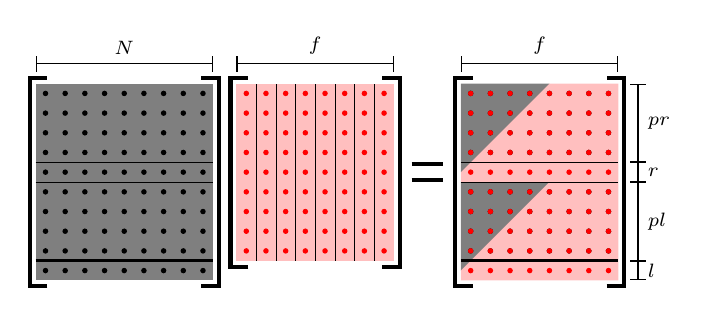
\begin{tikzpicture}
    % defining constants
    \def\stepSize{0.25}
    \def\Nnum{9}
    \def\fnum{8}
    \def\pnum{4}
    
    % Defining lengths
    \newlength{\onelen}
    \setlength{\onelen}{\stepSize cm}
    \newlength{\BrCl}
    \setlength{\BrCl}{0.075cm}
    \newlength{\BrIn}
    \setlength{\BrIn}{0.15cm}
    \newlength{\plen}
    \setlength{\plen}{1cm}%{\pnum\stepSize cm}
    \newlength{\flen}
    \setlength{\flen}{2cm}%{\fnum*\stepSize cm}
    \newlength{\Nlen}
    \setlength{\Nlen}{2.25cm}%{\Nnum\stepSize cm}%should be 2*p+one
    \newlength{\MatClearance}
    \setlength{\MatClearance}{0.3cm}
    
    % grid lines for guidance
    % \draw[gray,step=0.5] (-0,-1) grid (9,3);

    % ======================= drawing data matrix =======================
    \path (0,-\onelen) coordinate (M1A);
    \path ([xshift=\Nlen]M1A) coordinate (M1B);
    \path ([yshift=2*\plen+2*\onelen]M1B) coordinate (M1C);
    \path ([xshift=-\Nlen]M1C) coordinate (M1D);
    \draw[line width=1.5pt] ([xshift=\BrIn,yshift=-\BrCl]M1A) -- ([xshift=-\BrCl,yshift=-\BrCl]M1A) -- ([xshift=-\BrCl,yshift=\BrCl]M1D) -- ([xshift=\BrIn,yshift=\BrCl]M1D); %left bracket
    \draw[line width=1.5pt] ([xshift=-\BrIn,yshift=-\BrCl]M1B) -- ([xshift=\BrCl,yshift=-\BrCl]M1B) -- ([xshift=\BrCl,yshift=\BrCl]M1C) -- ([xshift=-\BrIn,yshift=\BrCl]M1C); %right bracket
    \draw[line width=1pt] ([yshift=\onelen]M1A) -- ([yshift=\onelen]M1B); % dividing matrix into blocks
    \fill[black, opacity=0.5] (M1A) rectangle (M1C);
    \foreach \x in {0,...,8} { % drawing black dots
    \foreach \y in {-1,...,8} {
      \fill ( {(\x+0.5)*\onelen}, {(\y+0.5)*\onelen} ) circle (1pt);
    }}
    \draw[line width=0.1pt] ([yshift=-\plen-\onelen]M1D) -- ([yshift=-\plen-\onelen]M1C);
    \draw[line width=0.1pt] ([yshift=-\plen]M1D) -- ([yshift=-\plen]M1C);
    
    % ======================= drawing G =======================
    % useful coordinates
    \path ([xshift=\MatClearance,yshift=\onelen]M1B) coordinate (M2A);
    \path ([xshift=\flen]M2A) coordinate (M2B);
    \path ([yshift=\Nlen]M2B) coordinate (M2C);
    \path ([xshift=-\flen]M2C) coordinate (M2D);

    % brackets
    \draw[line width=1.5pt] ([xshift=\BrIn,yshift=-\BrCl]M2A) -- ([xshift=-\BrCl,yshift=-\BrCl]M2A) -- ([xshift=-\BrCl,yshift=\BrCl]M2D) -- ([xshift=\BrIn,yshift=\BrCl]M2D); %left bracket
    \draw[line width=1.5pt] ([xshift=-\BrIn,yshift=-\BrCl]M2B) -- ([xshift=\BrCl,yshift=-\BrCl]M2B) -- ([xshift=\BrCl,yshift=\BrCl]M2C) -- ([xshift=-\BrIn,yshift=\BrCl]M2C); %right bracket
    
    % red fill
    \fill[red!50,opacity=0.5] (M2A) rectangle (M2C);

    % drawing red dots
    \foreach \x in {0,...,7} {
    \foreach \y in {0,...,8} {
      \fill[red] ([xshift=(\x+0.5)*\onelen,yshift=(\y+0.5)*\onelen]M2A) circle (1pt);%{(\x+0.5)*\onelen+\Nlen+0.5cm}, {(\y+0.5)*\onelen}
    }}

    % dividers
    \foreach \x in {1,...,7}{\draw[line width=0.1pt] ([xshift=\x*\onelen]M2A) -- ([xshift=\x*\onelen]M2D);}
    
    % ======================= drawing equal sign ======================= 
    \path ([xshift=\MatClearance*3/4,yshift=\Nlen/2-0.1cm]M2B) coordinate (EqA);
    \path ([xshift=0.4cm]EqA) coordinate (EqB);
    \path ([yshift=0.2cm]EqB) coordinate (EqC);
    \path ([xshift=-0.4cm]EqC) coordinate (EqD);
    \draw[line width = 1.5 pt] (EqA) -- (EqB);
    \draw[line width = 1.5 pt] (EqD) -- (EqC);

    % ======================= drawing RHS =======================
    % inside of matrix
    \path ([xshift=\MatClearance*3/4,yshift=-\Nlen/2+0.1cm-\onelen]EqB) coordinate (M3A);
    \path ([xshift=\flen]M3A) coordinate (M3B);
    \path ([yshift=2*\plen+2*\onelen]M3B) coordinate (M3C);
    \path ([xshift=-\flen]M3C) coordinate (M3D);
    % top left black triangle
    \path ([yshift=-\plen-\onelen/2]M3D) coordinate (t1A);
    \path ([xshift=\plen+\onelen/2]M3D) coordinate (t1B);
    % top red trapezoid
    \path ([yshift=-\onelen/2]t1A) coordinate (t2A);
    \path ([xshift=\flen]t2A) coordinate (t2B);
    % bottom black triangle
    \path ([yshift=-\plen-\onelen/2]t2A) coordinate (t3A);
    \path ([xshift=\plen+\onelen/2]t2A) coordinate (t3B);
    % bottom red trapezoid
    \path ([yshift=-\onelen/2]t3A) coordinate (t4A);

    % fill figures
    \fill[black, opacity=0.5]  (t1A) -- (t1B) -- (M3D) -- cycle;% top black
    \fill[red!50, opacity=0.5] (t2A) -- (t2B) -- (M3C) -- (t1B) -- (t1A) -- cycle;% top red
    \fill[black, opacity=0.5]  (t3A) -- (t3B) -- (t2A) -- cycle;% bottom black
    \fill[red!50, opacity=0.5] (t4A) -- (M3B) -- (t2B) -- (t3B) -- (t3A) -- cycle; % bottom red
    
    % draw brackets
    \draw[line width=1.5pt] ([xshift=\BrIn,yshift=-\BrCl]M3A) -- ([xshift=-\BrCl,yshift=-\BrCl]M3A) -- ([xshift=-\BrCl,yshift=\BrCl]M3D) -- ([xshift=\BrIn,yshift=\BrCl]M3D); %left bracket
    \draw[line width=1.5pt] ([xshift=-\BrIn,yshift=-\BrCl]M3B) -- ([xshift=\BrCl,yshift=-\BrCl]M3B) -- ([xshift=\BrCl,yshift=\BrCl]M3C) -- ([xshift=-\BrIn,yshift=\BrCl]M3C); %right bracket
    \draw[line width=1pt] ([yshift=\onelen]M3A) -- ([yshift=\onelen]M3B);
    
    % U_{i,p,N}
    \path ([xshift=0.5*\onelen,yshift=-\plen+0.5*\onelen]M3D) coordinate (tlbA);
    \foreach \x in {0,...,7}{
    \foreach \y in {0,...,3}{
        \ifthenelse{{\y>\x}\OR{\y=\x}}{%
        \fill[black] ([xshift={\x*\onelen},yshift={\y*\onelen}]tlbA) circle (1pt);%<do this if true>
        }{%
        \fill[red] ([xshift={\x*\onelen},yshift={(\y*\onelen}]tlbA) circle (1pt);%<do this if false>
        }%
    }}
    
    % U_{i_p,1,N}
    \path ([yshift=-\onelen]tlbA) coordinate (tlbB);
    \foreach \x in {0,...,7}{\fill[red] ([xshift=\x*\onelen]tlbB) circle (1pt);}
    
    % Y_{i,p,N}
    \path ([yshift=-\plen]tlbB) coordinate (tlbC);
    \foreach \x in {0,...,7}{
    \foreach \y in {0,...,3}{
        \ifthenelse{{\y>\x}\OR{\y=\x}}{%
        \fill[black] ([xshift={\x*\onelen},yshift={\y*\onelen}]tlbC) circle (1pt);%<do this if true>
        }{%
        \fill[red] ([xshift={\x*\onelen},yshift={(\y*\onelen}]tlbC) circle (1pt);%<do this if false>
        }%
    }}

    % Y_{i_p,1,N}
    \path ([yshift=-\onelen]tlbC) coordinate (tlbD);
    \foreach \x in {0,...,7}{\fill[red] ([xshift=\x*\onelen]tlbD) circle (1pt);}

    % draw dividers
    \draw[line width=0.1pt] ([yshift=-\plen-\onelen]M3D) -- ([yshift=-\plen-\onelen]M3C);
    \draw[line width=0.1pt] ([yshift=-\plen]M3D) -- ([yshift=-\plen]M3C);

    % ======================= length indicators ======================= 
    \draw[|-|] ([yshift=\onelen]M1D) -- node[above] {\scriptsize$N$} ([yshift=\onelen]M1C);
    \draw[|-|] ([yshift=\onelen]M2D) -- node[above] {\scriptsize$f$} ([yshift=\onelen]M2C);
    \draw[|-|] ([yshift=\onelen]M3D) -- node[above] {\scriptsize$f$} ([yshift=\onelen]M3C);
    \draw[|-|] ([xshift=\onelen]M3C) -- node[right] {\scriptsize$pr$} ([xshift=\onelen,yshift=\onelen]t2B);
    \draw[|-|] ([xshift=\onelen,yshift=\onelen]t2B) -- node[right] {\scriptsize$r$} ([xshift=\onelen]t2B);
    \draw[|-|] ([xshift=\onelen]t2B) -- node[right] {\scriptsize$pl$} ([xshift=\onelen,yshift=\onelen]M3B);
    \draw[|-|] ([xshift=\onelen,yshift=\onelen]M3B) -- node[right] {\scriptsize$l$} ([xshift=\onelen]M3B);
\end{tikzpicture}
\caption{Visualization of known (black) and unknown (red) variables in the \ac{CL-DeePC} framework given by \ref{eq:CL_DeePC_no_IVs}. Each dot represents a 'block' of inputs $u_k$, outputs $y_k$, or element of the matrix G.}
\label{fig:CL-DeePC}
\end{figure}
